\chapter{HASIL DAN PEMBAHASAN}
\section{Hasil}
\noindent

Tahapan ini merupakan tahapan yang berisi tentang penjelasan bagaimana game ini dapat bekerja sesuai dengan yang diharapkan dan dapat berjalan dengan baik. Tahapan ini meliputi perancangan perangkat lunak, bagian program yang penting dan implementasi sehingga dapat dipahami dengan baik dan mengetahui cara menggunakannya.

\subsection{Desain Perangkat Lunak}

\begin{enumerate}
    \item Tampilan \textit{Connecting Network} \\
    Tampilan \textit{connecting network} adalah tampilan awal disaat game dibuka, pada tampilan ini akan menghubungkan player ke jaringan photon .
    \begin{figure}[h]
        \centering
        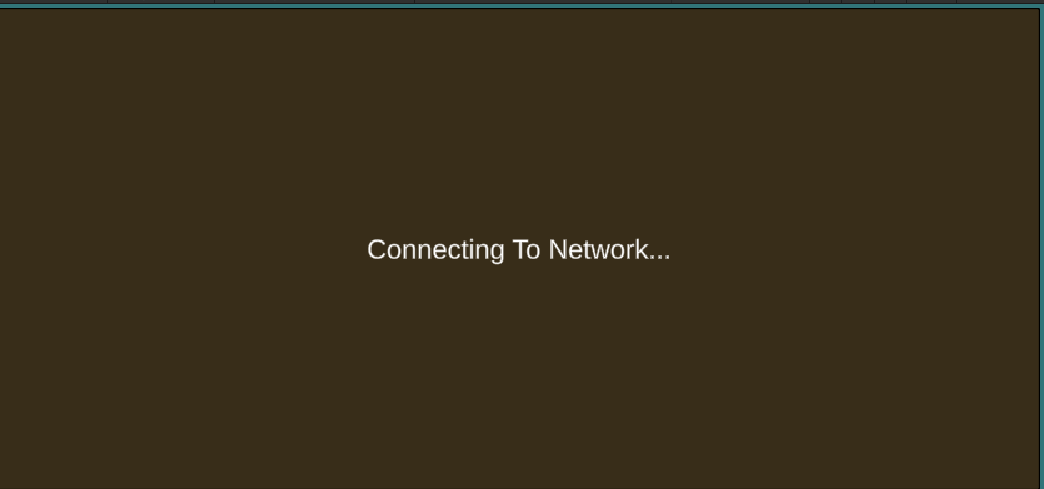
\includegraphics[width=10cm]{connecting.png}
        \caption{Tampilan \textit{Connecting Network}}
        \label{fig:connecting}
    \end{figure}
    \item Tampilan Set \textit{Nickname} \\
    Set \textit{nickname menu} merupakan letak dimana player harus mengisikan nama untuk memberikan identitas nama dari player. 
    \newpage
    \begin{figure}[h]
        \centering
        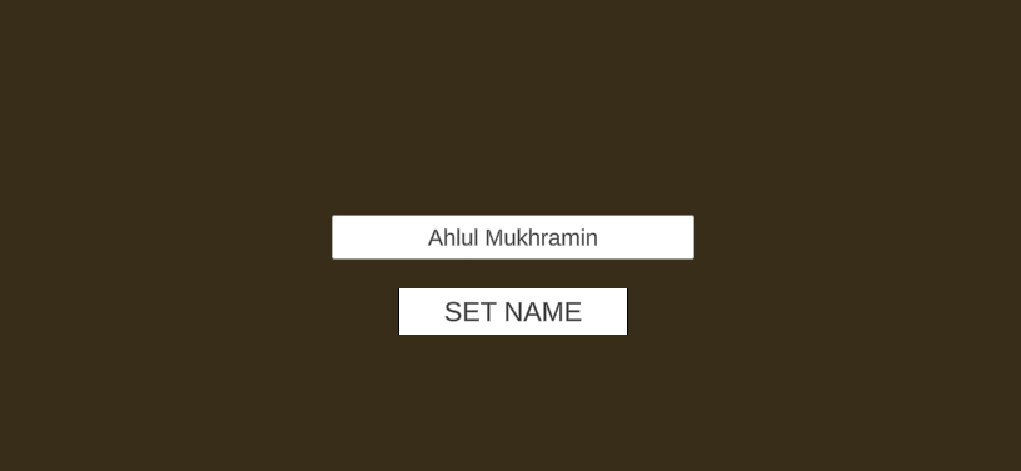
\includegraphics[width=10cm]{setnama.png}
        \caption{Tampilan Mengatur Nama}
        \label{fig:setnama}
    \end{figure}
    \item Tampilan Menu Utama\\
    Tampilan menu utama adalah tampilan menu yang terdapat button "cari room" untuk mencari room yang tersedia, "buat room" untuk membuat room sebagai master room,  "thanks to" untuk melihat \textit{credit} asset yang digunakan dan "Keluar" untuk menutup game.
    \begin{figure}[h]
        \centering
        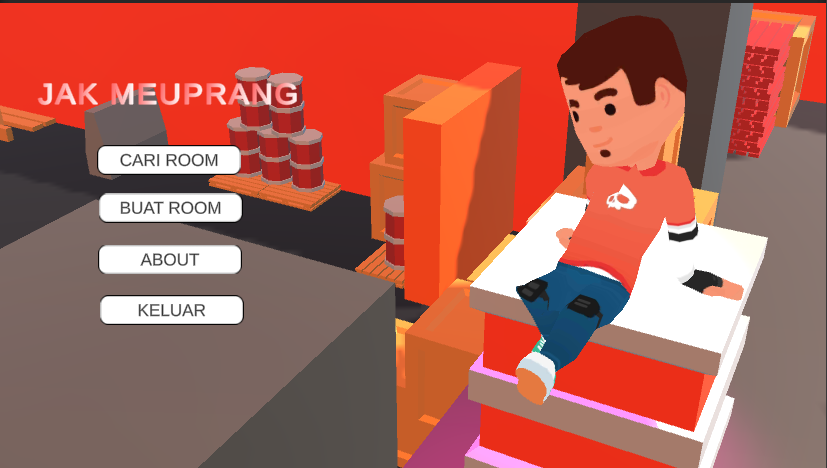
\includegraphics[width=10cm]{menuutama.png}
        \caption{Tampilan Menu Utama}
        \label{fig:menutama}
    \end{figure}
    \item Tampilan Pencarian Room\\
    Pencarian room merupakan menu untuk mencari room yang tersedia yang dibuat oleh player lain untuk memainkan game bersama.
    \newpage
    \begin{figure}[h]
        \centering
        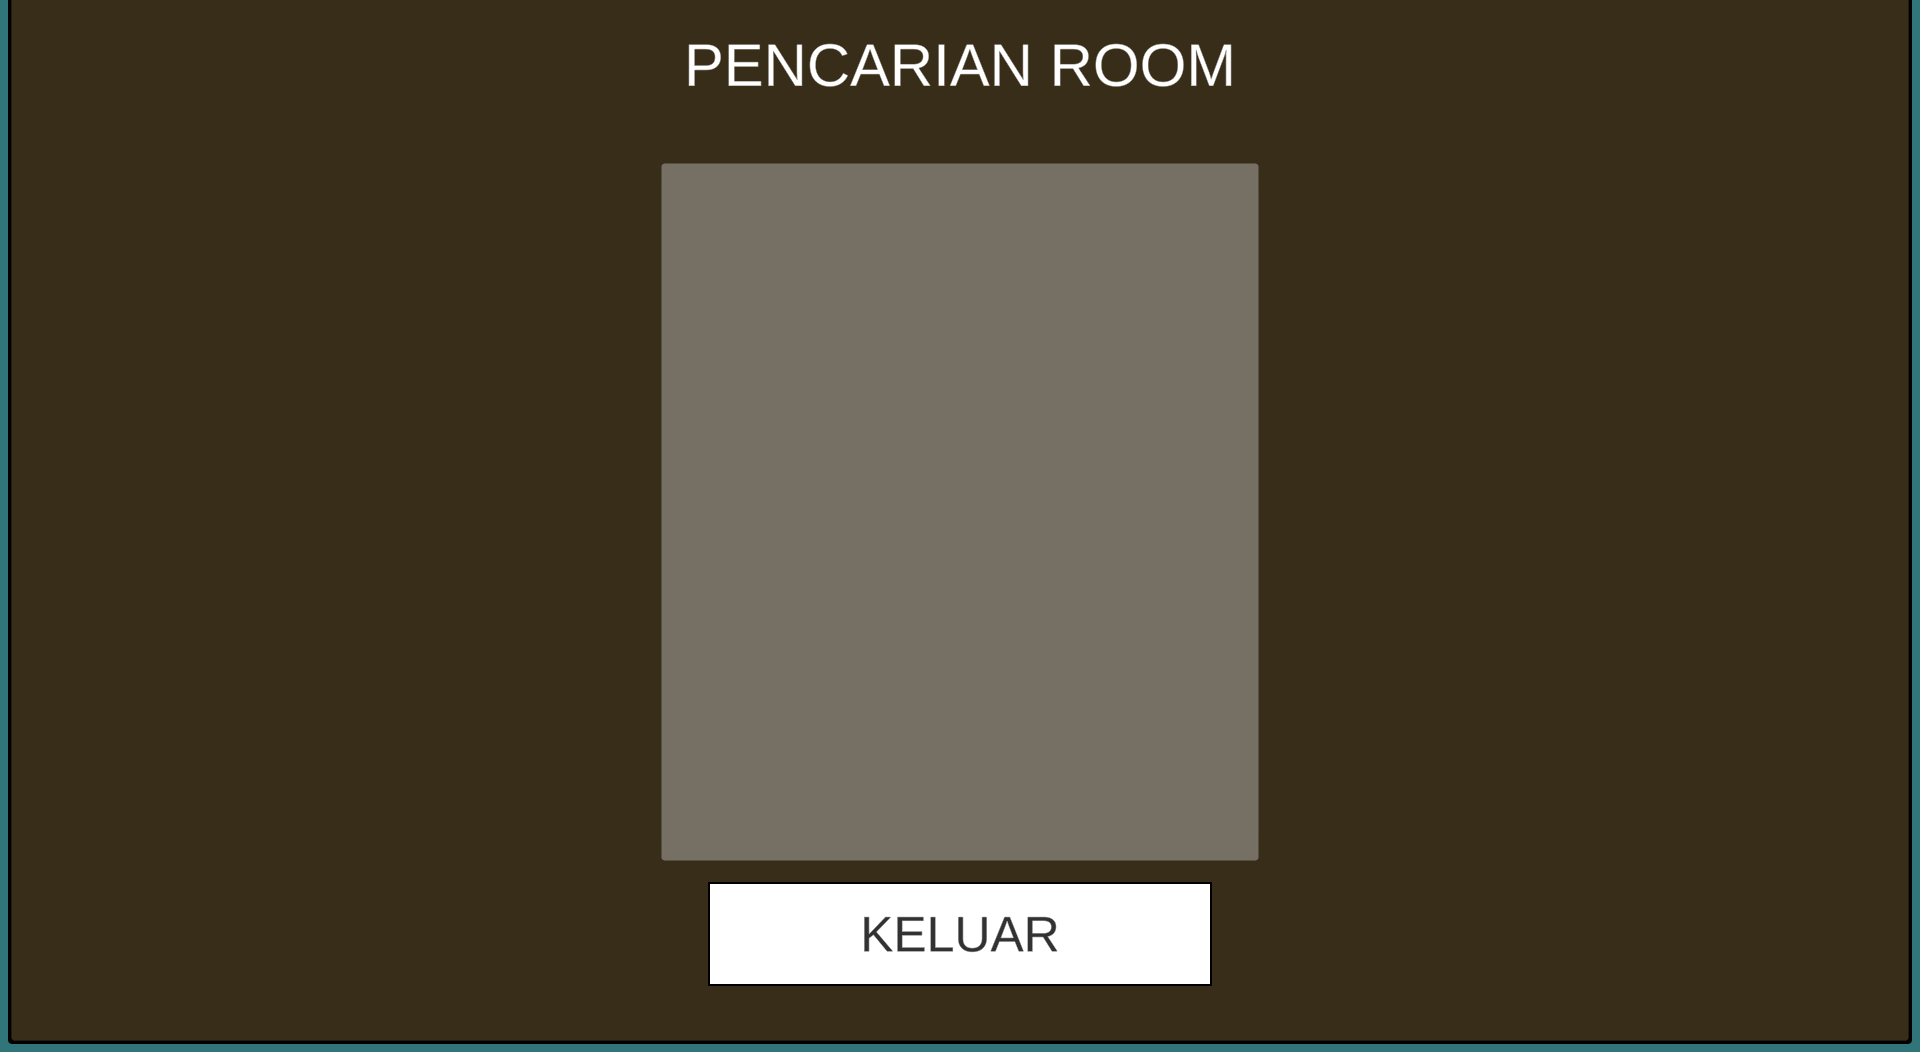
\includegraphics[width=10cm]{pencarian.png}
        \caption{Tampilan Pencarian}
        \label{fig:pencarian}
    \end{figure}
    \item Tampilan Buat Room \\
    Buat room merupakan menu untuk membuat room bagi player ingin menjadi host pada room tersebut, pada menu buat room ini player harus mengisikan nama room terlebih dahulul seperti gambar \ref{fig:namaroom}.
    \begin{figure}[h]
        \centering
        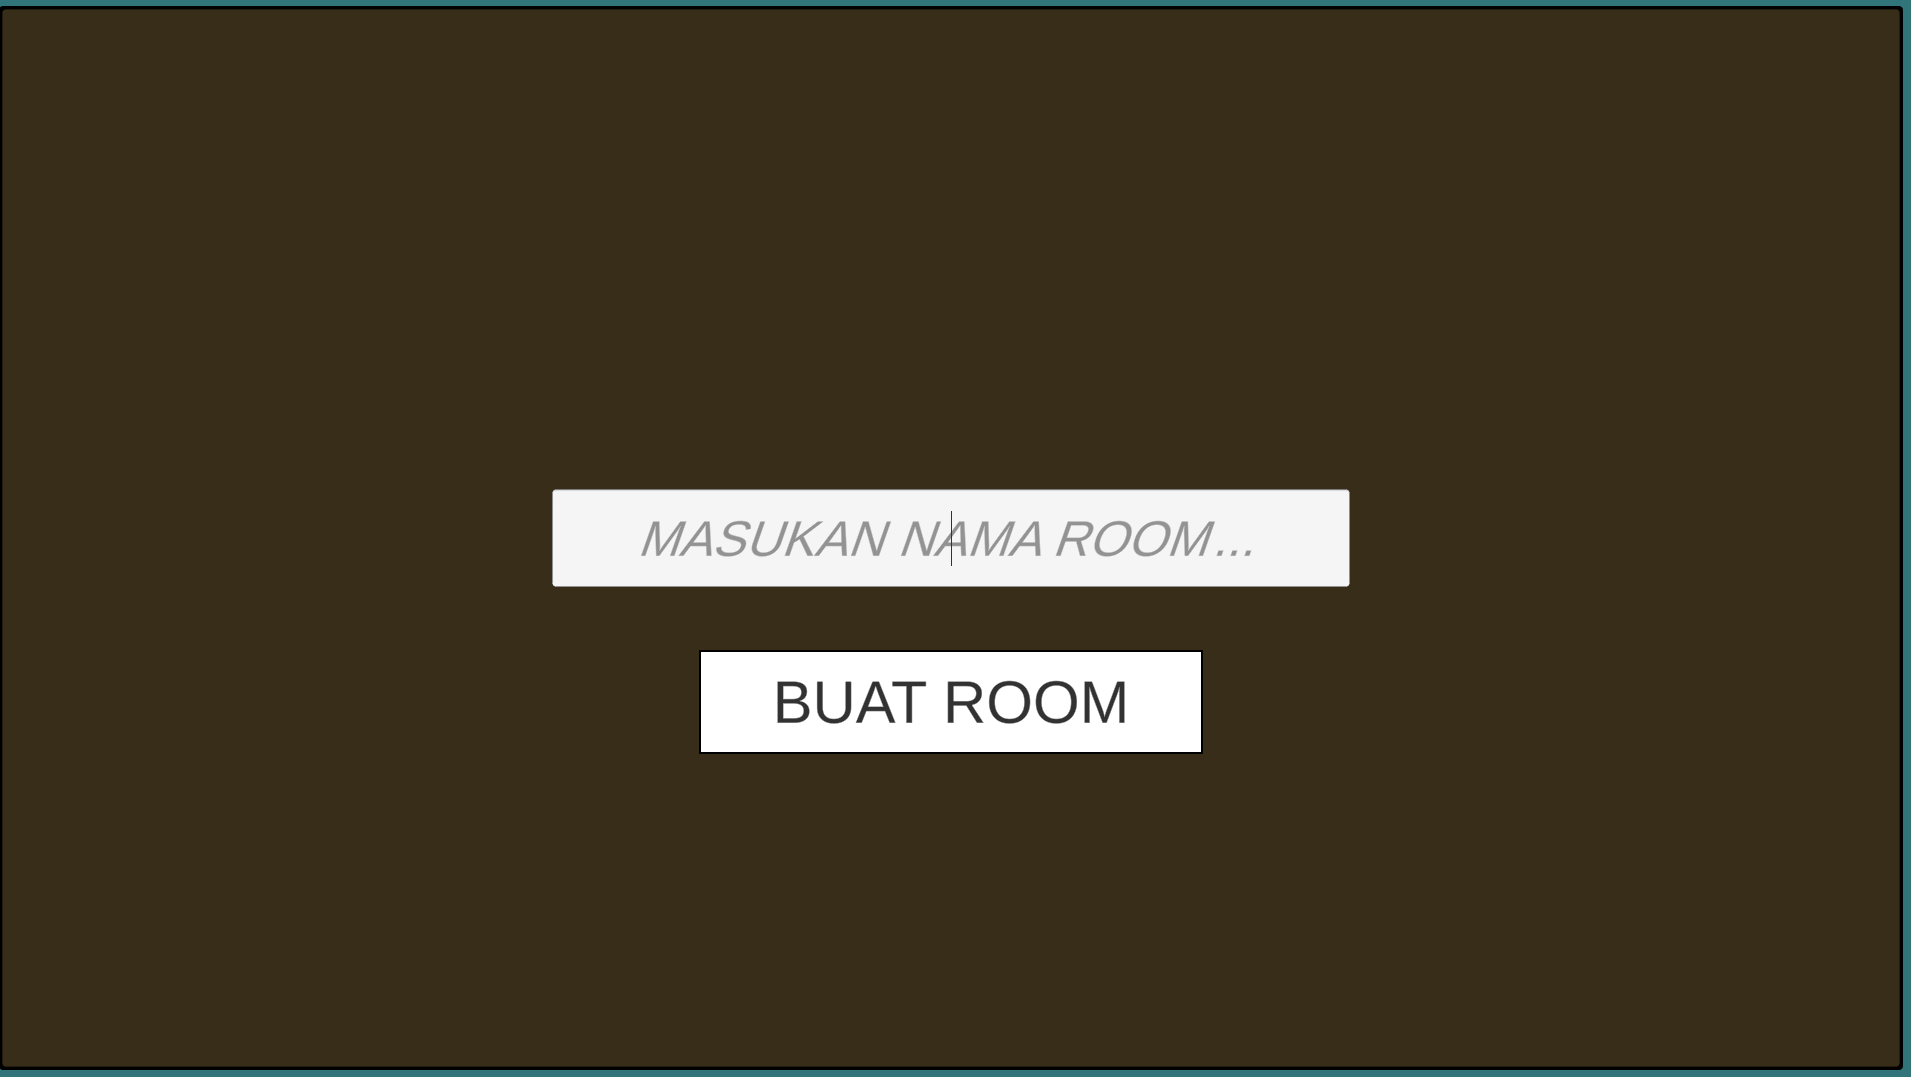
\includegraphics[width=10cm]{namaroom.png}
        \caption{Tampilan Buat Nama Room}
        \label{fig:namaroom}
    \end{figure}
    \\ setelah player telah mengisikan nama room maka akan menampilkan \textit{instance} baru yang berisi player player pada room tersebut, dan hanya host room yang dapat memulai permainannya.
    \newpage
    \begin{figure}[h]
        \centering
        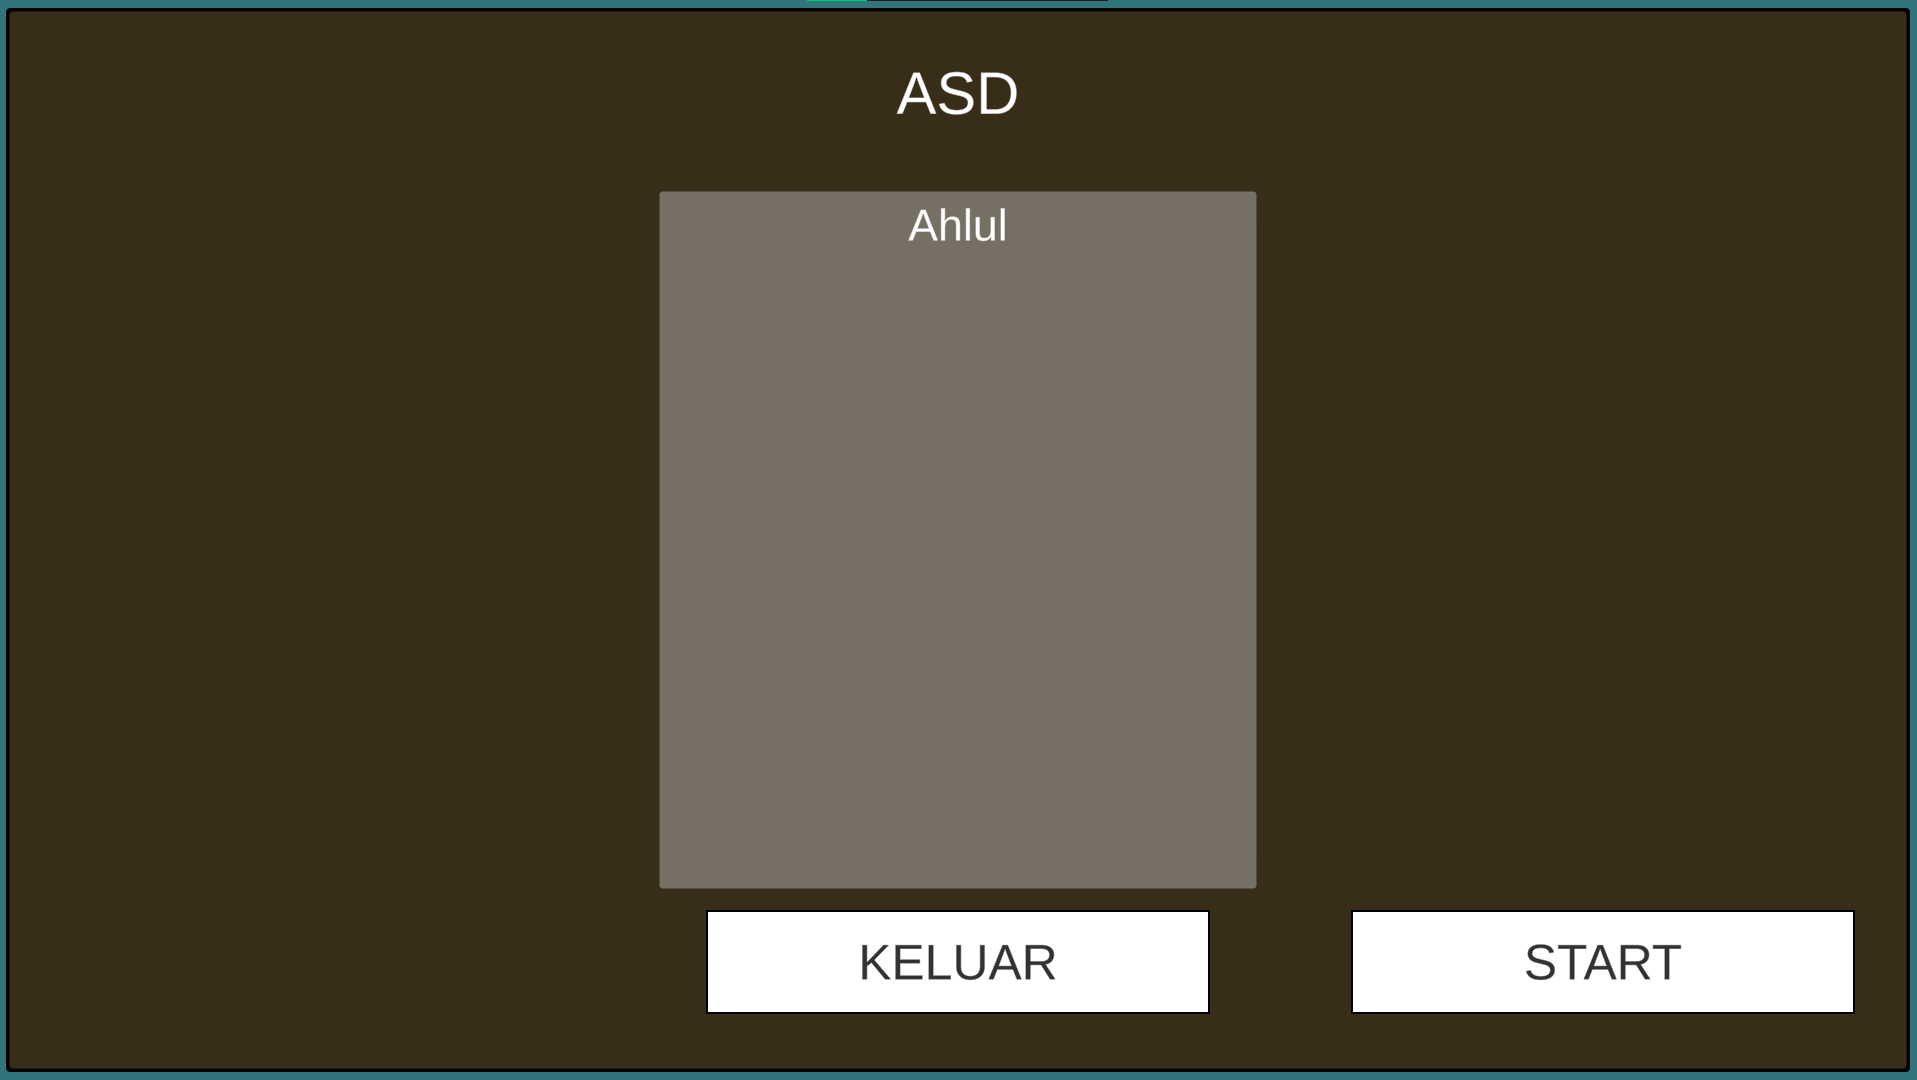
\includegraphics[width=10cm]{roomdone.png}
        \caption{Tampilan Room Telah Dibuat}
        \label{fig:roomdone}
    \end{figure}
    \item Tampilan Credit/About \\
    Tampilan ini merupakan tampilan informasi dari asset asset mana saja yang digunakan sebagai informasi.
    \begin{figure}[h]
        \centering
        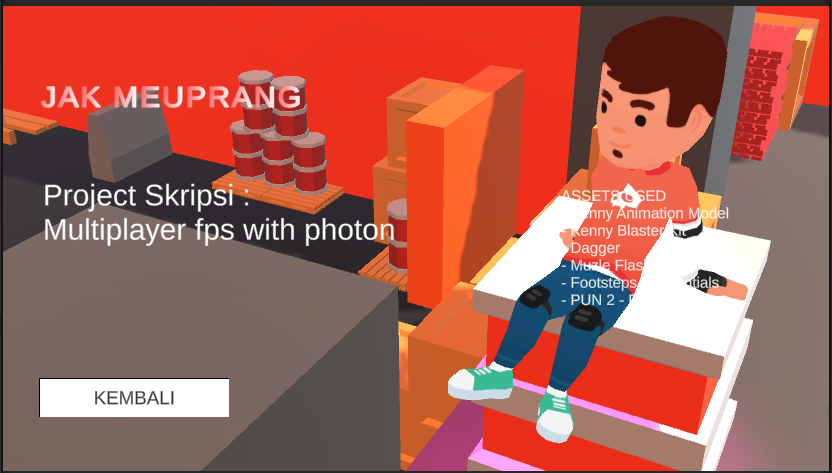
\includegraphics[width=10cm]{thanksto.png}
        \caption{Tampilan About}
        \label{fig:thanksto}
    \end{figure}
    \item Tampilan Gameplay \\
    Tampilan gameplay berisi permainan yang merupakan bagian area gameplay, pada tampilan gameplay ini menampilkan \textit{head up display} (HUD) seperti tampilan health, weapon overheat, player lain dan leaderboard.
    \newpage
    \begin{figure}[h]
        \centering
        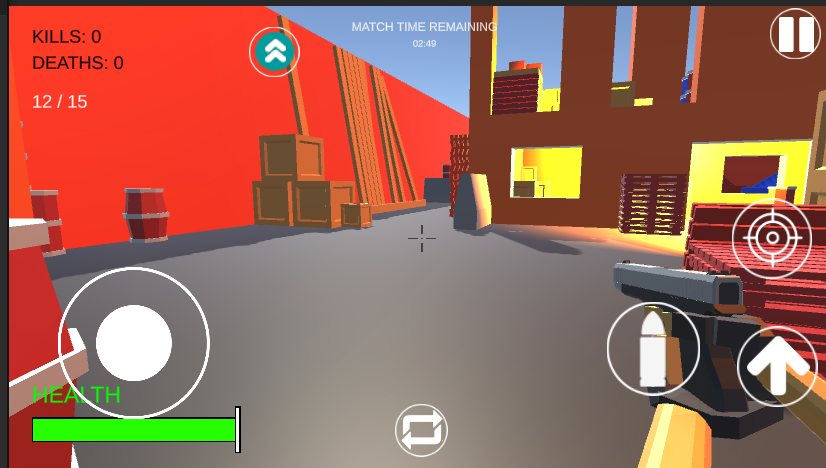
\includegraphics[width=10cm]{gameplay.png}
        \caption{Tampilan Gameplay}
        \label{fig:gameplay}
    \end{figure}
    \item Tampilan Round Over \\
    Tampilan ini ditampilkan jika waktu yang sudah ditentukan habis maka permainan telah berakhir dan player harus keluar untuk membuat room baru.
    \begin{figure}[h]
        \centering
        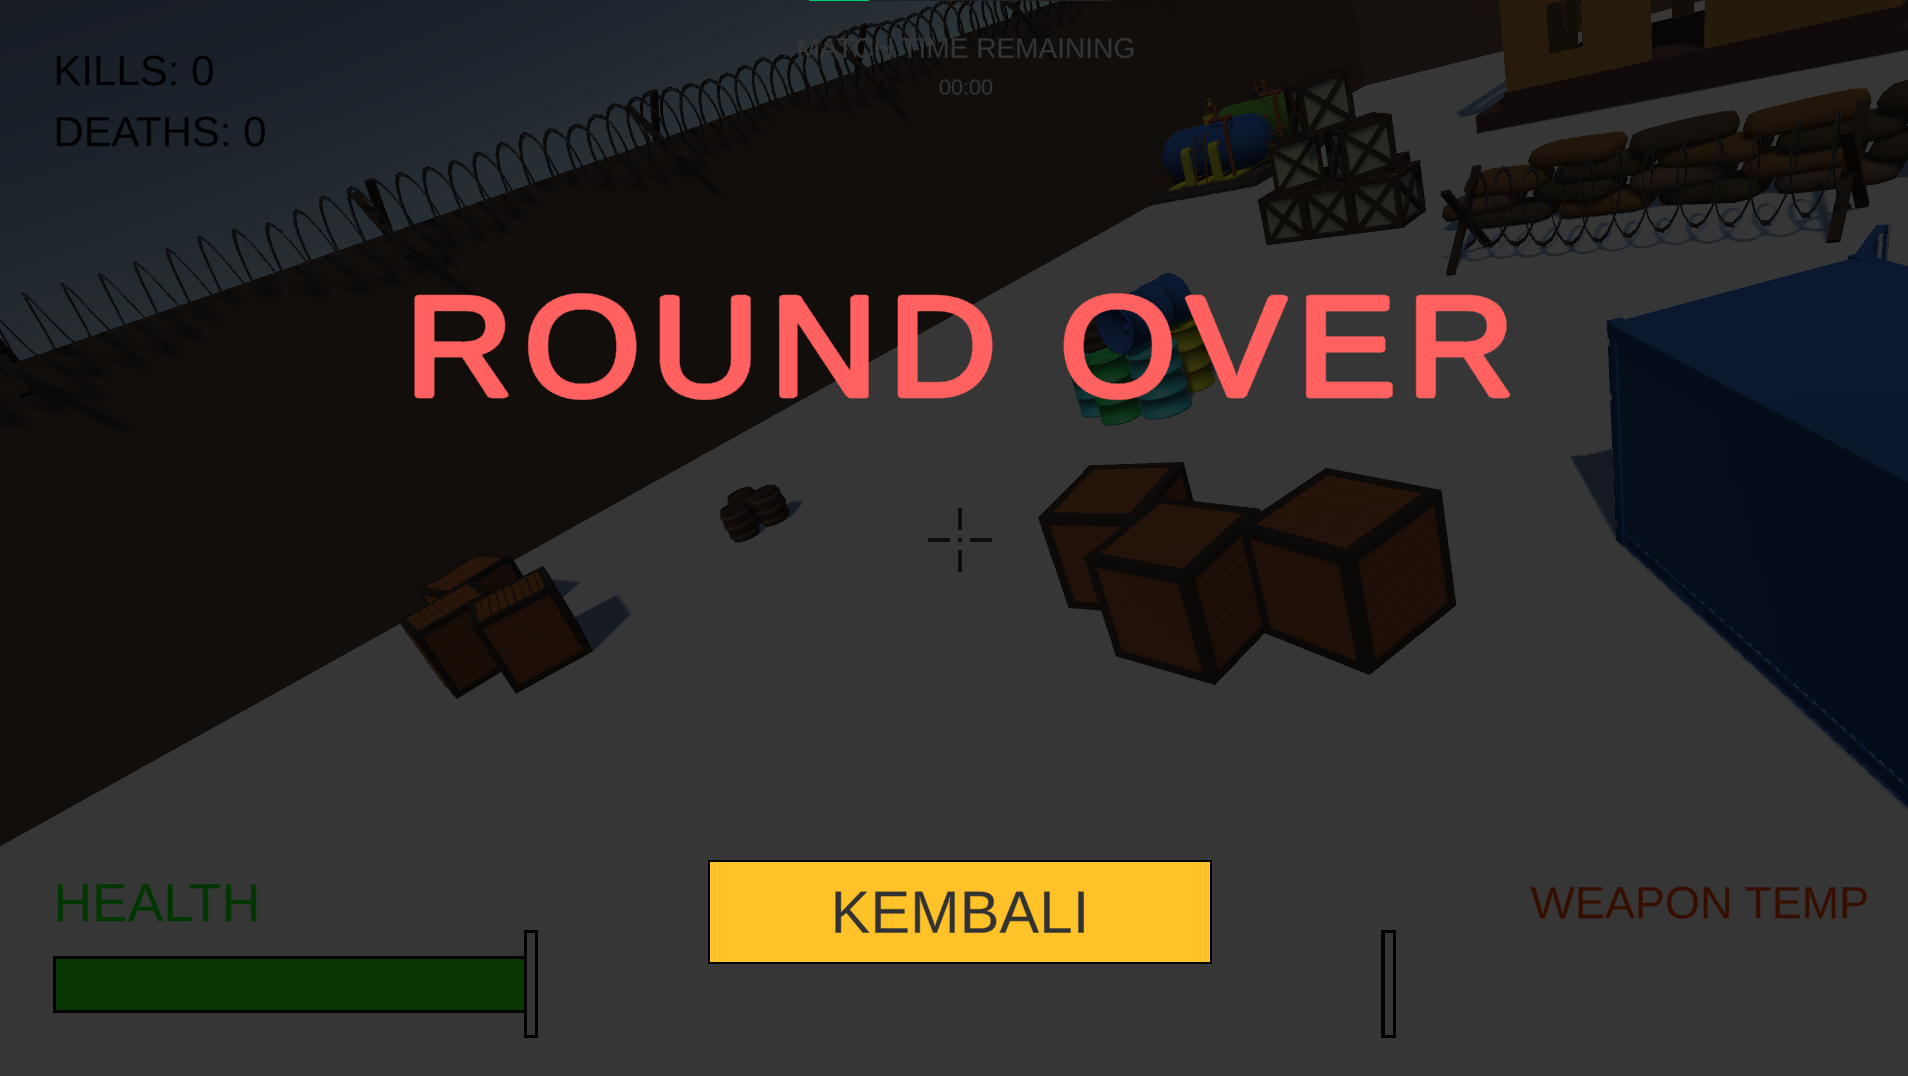
\includegraphics[width=10cm]{roundover.png}
        \caption{Tampilan Round Over}
        \label{fig:roundover}
    \end{figure}
\end{enumerate}